\documentclass{beamer}
% \documentclass[handout,t]{beamer}
\let\Tiny=\tiny

\batchmode
% \usepackage{pgfpages}
% \pgfpagesuselayout{4 on 1}[letterpaper,landscape,border shrink=5mm]

\usepackage[T1]{fontenc}
\usepackage{amsmath}
\usepackage{amssymb}
\usepackage{bbm}
\usepackage{beramono}
\usepackage{calc}
\usepackage{capt-of}
\usepackage{color}
\usepackage{enumerate}
\usepackage{epsfig}
\usepackage{expl3}
\usepackage{float}
\usepackage{graphicx}
\usepackage{hyperref}
\usepackage{ifthen}
\usepackage{listings}
\usepackage{lmodern}
\usepackage{pgfplots}
\usepackage{tikz-uml}
\usepackage{tikz}
\usepackage{upquote}
\usepackage{url}
\usepackage[utf8]{inputenc}
\usepackage{xcolor}

\usetheme{Berlin}
\usecolortheme{cin}

\lstset{
  aboveskip=15pt,
  basicstyle=\scriptsize,
  belowskip=0pt,
  captionpos=b,
  columns=fullflexible,
  extendedchars=true,
  frame=lines,
  framexbottommargin=4pt,
  framexleftmargin=17pt,
  framexrightmargin=5pt,
  numbers=left,
  numbersep=10pt,
  numberstyle=\tiny,
  showstringspaces=false,
  tabsize=2
}

\definecolor{wblue}{HTML}{3366CC}
\definecolor{wred}{HTML}{DC3912}
\definecolor{worange}{HTML}{FF9900}
\definecolor{wpurple}{HTML}{9F4C7C}

% cover -----------------------------------------------------------------------
\title{Tracking Library for the Web}
\author{Eduardo A. Lundgren Melo}
\institute[CIn/UFPE]{
    \scalebox{2}{
        \includegraphics[height=.07\textheight]{ufpe-logo.png}
        \quad
        \includegraphics[height=.07\textheight]{cin-logo.png}
    }
}
\date{{\bf Master of Science in Computer Science}\\
\vspace{0.5cm}
{\footnotesize
Silvio de Barros Melo (\emph{Advisor})\\
Veronica Teichrieb (\emph{Co-Advisor})}}
% cover end -------------------------------------------------------------------

\pgfdeclareimage[height=0.5cm]{cin-logo}{cin-logo.png}
\logo{\pgfuseimage{cin-logo}\hspace*{0.3cm}}

\AtBeginSection[]
{
  \begin{frame}<beamer>
    \frametitle{Outline}
    \tableofcontents[currentsection]
  \end{frame}
}
\beamerdefaultoverlayspecification{<+->}

% -----------------------------------------------------------------------------
\begin{document}
% -----------------------------------------------------------------------------

\frame{\titlepage}

\section[Outline]{}
\begin{frame}{Outline}
  \tableofcontents
\end{frame}

% -----------------------------------------------------------------------------
\section{Introduction}
\begin{frame}{Motivation}
  \begin{itemize}
    \item The web browser environment is evolving fast
    \item Phones and notebooks devices have embedded web browser
    \item Entertainment solutions are gaining space on the web
    \item Vision is an accurate and low-cost solution
  \end{itemize}
\end{frame}
\begin{frame}{Problem definition}
  \begin{itemize}
    \item JavaScript is a language interpreted by all web browsers
    \item Interpreted languages have limited computational power
    \item Modern web browsers can natively capture the user media
    \item Capturing and processing user media are required steps for visual tracking
  \end{itemize}
\end{frame}
\begin{frame}{Objectives}
  \begin{itemize}
    \item Facilitate user interaction with the web browser
    \item Accelerate the use of visual tracking in commercial products
    \item Provide a cross-platform tracking library
    \item Design and implement a tracking library for the web
  \end{itemize}
\end{frame}
% -----------------------------------------------------------------------------
\section{Basic concepts}

\subsection{Web}
\begin{frame}{World Wide Web}
  \begin{block}{}
      The World Wide Web is a shared information system operating on top of the Internet
  \end{block}
\end{frame}
\begin{frame}{The beggining of the web}
  \begin{itemize}
    \item Plain text and images were the most advanced features
    \item In 1994, the World Wide Web Consortium (W3C) was founded
    \item Companies were able to contribute to the W3C specifications
    \item Today's web is a result of the ongoing efforts of an open web
  \end{itemize}
\end{frame}
\begin{frame}{The modern web}
  \begin{itemize}
    \item Contributions transformed the web in a growing universe
    \item Videos, audio, photos, interactive content, 3D graphics
    \item Processed by the Graphics Processing Unit (GPU)
    \item Without requiring any third-party plugins installation
  \end{itemize}
\end{frame}
\begin{frame}{Browser technologies}
  \begin{itemize}
    \item Web pages are written using HyperText Markup Language
    \item Web can be augmented with other technologies
    \item JavaScript is the main programming language
    \item Layout and style information uses Cascading Style Sheets
  \end{itemize}
\end{frame}
\begin{frame}{Browser architecture}
  \begin{figure}[!htb]
    \centering
    \includegraphics[width=220pt]{../chapters/basic_concepts/web_architecture.pdf}
    \caption{Reference architecture for web browsers}
    \label{figure:web_architecture}
  \end{figure}
\end{frame}
\begin{frame}{Audio and video}
  \begin{figure}[!htb]
    \centering
    \includegraphics[width=220pt]{../chapters/basic_concepts/html5_audio_video.png}
    \caption{Video and audio HTML5 elements}
    \label{figure:html5_audio_video}
  \end{figure}
\end{frame}
\begin{frame}[fragile]{Audio and video}
\begin{lstlisting}[language=C++,label={lst:get_user_media},caption=Capturing browser microphone and camera]
  <video autoplay></video>
  <script>
    var video = document.querySelector('video');
    navigator.getUserMedia({video: true, audio: true}, function(localMediaStream) {
        video.src = window.URL.createObjectURL(localMediaStream);
        video.onloadedmetadata = function(e) { alert('Ready to go.') };
    }, onFail);
  </script>
  \end{lstlisting}
\end{frame}
\begin{frame}{Canvas element}
  \begin{itemize}
    \item HTML5 element
    \item Resolution-dependent bitmap canvas
    \item Two-dimensional grid, computer graphics coordinate system
    \item Can render graphs, game graphics, art, or other visual images
  \end{itemize}
\end{frame}
\begin{frame}{Canvas element}
  \begin{figure}[!htb]
    \centering
    \includegraphics[width=130pt]{../chapters/basic_concepts/canvas_axis.pdf}
    \caption{The canvas coordinate space}
    \label{figure:canvas_axis}
  \end{figure}
\end{frame}
\begin{frame}{JavaScript typed arrays}
  \begin{itemize}
    \item In the past, raw data was accessed as a string
    \item Browsers need to quickly manipulate raw binary data
    \item Typed data structures were added to JavaScript
    \item JavaScript-typed arrays access raw binary more efficiently
  \end{itemize}
\end{frame}
\begin{frame}{Typed arrays performance benchmark}
  \begin{figure}[!htb]
    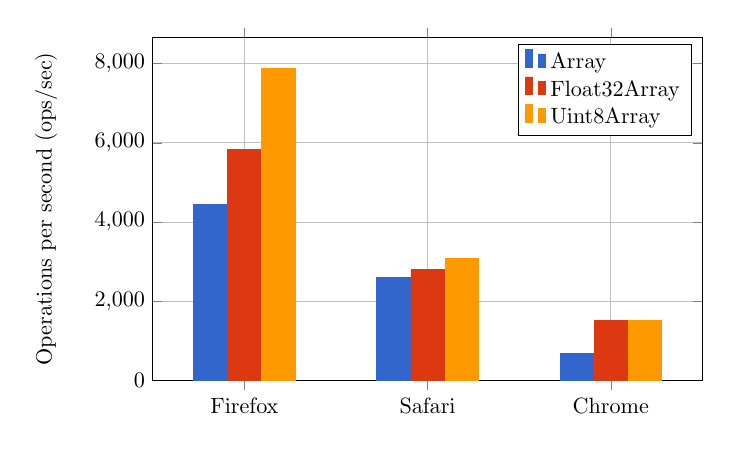
\begin{tikzpicture}[scale=0.8]
        \begin{axis}[
            bar width=15pt,
            enlarge x limits=0.25,
            height= 200pt,
            legend cell align=left,
            scaled y ticks=false,
            symbolic x coords={Firefox,Safari,Chrome},
            width=0.85*\textwidth,
            xmajorgrids=true,
            xtick=data,
            ybar=\pgflinewidth,
            ylabel={Operations per second (ops/sec)},
            ylabel style={yshift=10pt},
            ymajorgrids=true,
            ymin=0
        ]
            \addplot[style={wblue, fill=wblue}]
                coordinates {
                  (Firefox, 4437)
                  (Safari, 2607)
                  (Chrome, 679)
                };

            \addplot[style={wred, fill=wred}]
                coordinates {
                  (Firefox, 5841)
                  (Safari, 2797)
                  (Chrome, 1510)
                };

            \addplot[style={worange, fill=worange}]
                coordinates {
                  (Firefox, 7872)
                  (Safari, 3089)
                  (Chrome, 1510)
                };

            \legend{Array,Float32Array,Uint8Array}
        \end{axis}
    \end{tikzpicture}
    \caption{Regular \textit{vs} typed arrays performance benchmark}
    \label{figure:typed_arrays_performance}
  \end{figure}
\end{frame}
\begin{frame}{What is the relation between typed arrays and canvas?}
  \begin{itemize}
    \item Videos and images pixels can be drawn on a canvas bitmap
    \item Canvas raw binary data can be accessed from JavaScript
    \item Canvas array of pixels, is in row-major order
    \item Consider the $2\times3$ array $\begin{bmatrix}
1 & 2 & 3\\
4 & 5 & 6
\end{bmatrix}$, in row-major order it is laid out contiguously in linear memory as $\begin{bmatrix}
1 & 2 & 3 & 4 & 5 & 6
\end{bmatrix}$.
  \end{itemize}
\end{frame}
\begin{frame}{What is the relation between typed arrays and canvas?}
  \begin{figure}[!htb]
    \centering
    \includegraphics[width=\linewidth]{../chapters/basic_concepts/imagedata_array.pdf}
    \caption{The canvas image data array of pixels}
    \label{figure:imagedata_array}
  \end{figure}
\end{frame}
\begin{frame}{What is the relation between typed arrays and canvas?}
  \begin{figure}[!htb]
    \centering
    \includegraphics[width=240pt]{../chapters/basic_concepts/get_user_media.pdf}
    \caption{Access flow of raw binary data captured from videos on modern browsers}
    \label{figure:get_user_media}
  \end{figure}
\end{frame}

\subsection{Visual tracking}
\begin{frame}{Visual tracking}
  \begin{block}{}
      Tracking an object in a video sequence means continuously identifying its location when either the object or the camera are moving
  \end{block}
  \begin{figure}[!htb]
    \centering
    \includegraphics[width=\linewidth]{../chapters/basic_concepts/tracking_occlusion.png}
    \caption{Example of an accurate object tracking robust to occlusion}
    \label{figure:tracking_occlusion}
  \end{figure}
\end{frame}
\begin{frame}{Visual tracking}
  \begin{figure}[!htb]
    \centering
    \includegraphics[width=200pt]{../chapters/basic_concepts/cv_applications.png}
    \caption{Computer vision applications: motion-based recognition (top left); automated surveillance (top center); video indexing (top right); human-computer interaction (bottom left); traffic monitoring (bottom center); vehicle navigation (bottom right).}
    \label{figure:cv_applications}
  \end{figure}
\end{frame}

\begin{frame}{Which devices could use tracking.js?}
  \begin{block}{}
      Different devices such as mobile phones, notebooks, and even head-worn (Google Project Glass), provide an embedded web browser capable to run JavaScript and HTML5.
  \end{block}
\end{frame}
% % -----------------------------------------------------------------------------
\section{Tracking library for the web}

\begin{frame}{tracking.js}
  \begin{block}{}
      Tracking library for the web aiming to provide a common infrastructure to develop applications and to accelerate the use of those techniques on the web in commercial products
  \end{block}
  \begin{block}{}
      It runs on native web browsers without requiring third-party plugins installation
  \end{block}
\end{frame}
\begin{frame}{Related work}
  \begin{itemize}
    \item FLARToolKit: a port of the well-known ARToolKit marker tracking library to ActionScript
  \end{itemize}
  \begin{figure}[!htb]
    \centering
    \includegraphics[width=130pt]{../chapters/tracking_library_for_the_web/flartoolkit.png}
    \caption{Marker based AR for the web using FLARToolKit}
    \label{figure:flartoolkit}
  \end{figure}
\end{frame}
\begin{frame}{Related work}
  \begin{itemize}
    \item JSARToolkit: is a JavaScript port of FLARToolKit
  \end{itemize}
  \begin{figure}[!htb]
    \centering
    \includegraphics[width=130pt]{../chapters/tracking_library_for_the_web/jsartoolkit.png}
    \caption{Marker-based AR for the web using JSARToolKit}
    \label{figure:jsartoolkit}
  \end{figure}
\end{frame}
\begin{frame}{Related work}
  \begin{itemize}
    \item Unifeye Viewer: from Metaio company, it offers a robust markerless tracking solution for the web to ActionScript
  \end{itemize}
  \begin{figure}[!htb]
    \centering
    \includegraphics[width=130pt]{../chapters/tracking_library_for_the_web/unifeyeviewer.png}
    \caption{Markerless example of image projected over a magazine cover using Unifeye Viewer solution}
    \label{figure:unifeyeviewer}
  \end{figure}
\end{frame}
\begin{frame}{Library modules}
  \begin{figure}[!htb]
      \tikzumlset{font=\tiny}
      \begin{tikzpicture}
          \umlclass[x=100pt]{Math}{}

          \umlclass{Attribute}{}

          \umlclass[y=-50pt]{DOMElement}{}

          \umlclass[y=-85pt,x=-80pt]{Canvas}{}

          \umlclass[y=-110pt]{Video}{}

          \umlclass[y=-110pt,x=100pt]{VideoCamera}{}

          \umlinherit[geometry=-|]{DOMElement}{Attribute}
          \umlinherit[geometry=-|]{Canvas}{DOMElement}
          \umlinherit[geometry=-|]{Video}{DOMElement}
          \umlinherit[geometry=|-]{VideoCamera}{Video}
      \end{tikzpicture}
      \caption{Base classes of tracking.js library}
      \label{figure:base_classes}
  \end{figure}
\end{frame}
\begin{frame}{Library modules}
  \begin{figure}[!htb]
      \tikzumlset{font=\tiny}
      \begin{tikzpicture}
          \umlclass{FAST}{}{
            findCorners(data, threshold) : Array\\
          }

          \umlclass[y=-55pt]{BRIEF}{}{
            getDescriptors(data, corners) : Array\\
            match(c1, d1, c2, d2) : Array\\
          }

          \umlclass[y=-110pt]{ViolaJones}{}{
            find() : Array\\
            evalStage() : boolean\\
          }

          \umlclass[y=-110pt,x=140pt]{Color}{}{
            find() : Array\\
          }

          \umlclass[x=140pt]{RANSAC}{}{
            find(matches) : void\\
            score() : Number\\
          }

          \umlclass[y=-55pt,x=140pt]{Homography}{}{
              score(H, matches) : Number\\
          }

          \umlinherit[geometry=-|]{Homography}{RANSAC}
      \end{tikzpicture}
      \caption{Visual tracking classes of tracking.js library}
      \label{figure:visual_tracking_classes}
  \end{figure}
\end{frame}
\begin{frame}{Feature detector}
  \begin{itemize}
    \item Detects individual features (\textit{keypoints}) across images
    \item Robustness against partial occlusions or matching errors
    \item Used as the first step of many vision tasks such as tracking
    \item Features from Accelerated Segment Test (FAST)
  \end{itemize}
\end{frame}
\begin{frame}{Feature detector}
  \begin{figure}[!htb]
    \centering
    \includegraphics[width=220pt]{../chapters/tracking_library_for_the_web/keypoints.png}
    \caption{Image features detected on two different frames, green pixels represents found keypoints}
    \label{figure:keypoints}
  \end{figure}
\end{frame}
\begin{frame}{Feature detector}
  \begin{block}{Features from Accelerated Segment Test (FAST)}
      It works by testing a small patch of an image to see if it could be a corner
  \end{block}
  \begin{block}{}
      The detector is evaluated using a circle surrounding the candidate pixel
  \end{block}
  \begin{block}{}
      The test is based on whether the concentric contiguous arcs around the pixel are significantly different from the central pixel $p$
  \end{block}
\end{frame}
\begin{frame}{Feature detector}
  \begin{figure}[!htb]
    \centering
    \includegraphics[width=220pt]{../chapters/tracking_library_for_the_web/fast.png}
    \caption{FAST: point segment test corner detection in an image patch}
    \label{figure:fast}
  \end{figure}
\end{frame}
\begin{frame}{Feature detector}
  \begin{itemize}
    \item FAST technique was chosen for feature detector
    \item Robust against occlusions, matching errors and illumination
    \item Has excellent repeatability
    \item Computational complexity of the technique is low
  \end{itemize}
\end{frame}
\begin{frame}{Feature extractor}
  \begin{itemize}
    \item To estimate motion, match sets of features is required
    \item For each point \{$m_{i}$\} in the first image, search in a region of the second image around location \{$m_{i}$\} for point \{$m'_{j}$\}
    \item The search is based on the similarity of the local image windows
    \item Binary Robust Independent Elementary Features (BRIEF)
  \end{itemize}
\end{frame}
\begin{frame}{Feature extractor}
  \begin{figure}[!htb]
    \centering
    \includegraphics[width=220pt]{../chapters/tracking_library_for_the_web/BRIEF.pdf}
    \caption{Feature extractor}
    \label{figure:BRIEF}
  \end{figure}
\end{frame}
\begin{frame}{Feature extractor}
  \begin{block}{Binary Robust Independent Elementary Features (BRIEF)}
      Searches for correspondent points in the current frame and only points that are highly descriptive invariant features, called keypoints, are tested
  \end{block}
  \begin{block}{}
      After the keypoints are detected they need to be described and the respective matching point should be found
  \end{block}
  \begin{block}{}
      BRIEF uses a binary string to describe the keypoints and having local descriptors that are fast to compute, to match and being memory efficient are important aspects
  \end{block}
\end{frame}
\begin{frame}{Feature extractor}
  To generate the binary strings it is defined the test $\tau$ on patch \textbf{p} of size \textbf{S $\times$ S} as

  $$\tau(\textbf{p}; x, y) :=
  \begin{cases}
    1 &\mbox{if}\quad \textbf{p(x)} < \textbf{p(y)},\\
    0 &\mbox{otherwise}
  \end{cases}$$

  where \textbf{p(x)} is the pixel intensity. The set of binary tests is defined by the $n_{d}$ (\textbf{x}, \textbf{y})-location pairs uniquely chosen during the initialization
\end{frame}
\begin{frame}{Feature extractor}
  The $n_{d}$-dimensional bit-string is our BRIEF descriptor for each keypoint

  $$f_{n_{d}}(\textbf{p}) := \sum_{1 \le i \le n_{d}} 2^{i-1} \tau(\textbf{p}; x, y).$$

  In this work, $n_{d}= 128$ was used, since it presented good matching results and performance. The number of bytes required to store the descriptor can be calculated by $k = n_{d}/8$
\end{frame}
\begin{frame}{Feature extractor}
  \begin{itemize}
    \item Each keypoint is described with its binary string
    \item Each keypoint is compared with the closest matching point
    \item Distance metric is critical to the performance
    \item Using binary strings reduces the size of the descriptor
  \end{itemize}
\end{frame}
\begin{frame}{Feature extractor}
  Given two image patches $x$ and $y$, denote their binary descriptors as $b(x) \in \{0,1\}^n$ and $b(y) \in \{0,1\}^n$ respectively, the Hamming distance is computed by
  $$Ham(x, y)=\sum_{i=1}^{n}b_i(x)\otimes b_i(y)$$
  From the hamming distance, the Hamming weight can be calculated
  $$WHam(x, y)=\sum_{i=1}^{n}w_i(b_i(x)\otimes b_i(y))$$
\end{frame}
\begin{frame}{Feature extractor}
  \begin{itemize}
    \item BRIEF technique was chosen for feature extractor
    \item Use binary strings to describe the keypoints
    \item Fast to compute, to match and is memory efficient
    \item Computational complexity of the technique is low
  \end{itemize}
\end{frame}
\begin{frame}{Homography estimation}
  \begin{block}{}
      Homographies are estimated between images by finding feature correspondences on them
  \end{block}
  \begin{block}{}
      A 2D point $(x,y)$ in an image can be represented as a 3D vector $\textbf{x} = (x_1, x_2, x_3)$ where $x = \frac{x_1}{x_3}$ and $y = \frac{x_2}{x_3}$
  \end{block}
\end{frame}
\begin{frame}{Homography estimation}
  Homography is a mapping from $P^2$ → $P^2$ which is a projectivity if and only if there exists a non-singular $3\times3$ matrix $H$ such that for any point in $P^2$ represented by vector $\textbf{x}$ it is true that its mapped point equals $H\textbf{x}$

  $$c\begin{pmatrix}u\\ v\\ 1\\\end{pmatrix} = H\begin{pmatrix}x\\ y\\ 1\\\end{pmatrix}, \;\; H=\begin{pmatrix}h1 & h2 & h3\\ h4 & h5 & h6\\ h7 & h8 & h9\\\end{pmatrix},$$
  where $c$ is any non-zero constant, $(\; u \; v \; 1 \;)^T$ represents $\textbf{x'}$, $(\; x \; y \; 1 \;)^T$ represents $\textbf{x}$
\end{frame}
\begin{frame}{Random sample consensus (RANSAC)}
  \begin{block}{}
      RANSAC (Random Sample Consensus) is an iterative method to estimate parameters of a mathematical model from a set of observed data which contains outliers
  \end{block}
  \begin{block}{}
      It is the most commonly used robust estimation method for homographies
  \end{block}
\end{frame}
\begin{frame}{Random sample consensus (RANSAC)}
  The idea of the algorithm is pretty simple
  \pause
  \begin{itemize}
    \item<2-> For $N$ iterations, a random sample of $4$ correspondences is selected and $H$ is computed
    \item<3-> Each other correspondence is classified as an inlier or outlier
    \item<4-> The iteration containing more inliers is selected
    \item<5-> The matrix $H$ is recomputed from all inliers in that iteration
  \end{itemize}
\end{frame}
\begin{frame}{Rapid object detection (Viola Jones)}
  \begin{itemize}
    \item Robust and extremely rapid object detection
    \item Became popular mainly because rapid face detection
    \item A training phase is required
    \item A scanning detector is what makes the detection
  \end{itemize}
\end{frame}
\begin{frame}{Rapid object detection (Viola Jones)}
  \begin{block}{Features}
      Images are classified based on the value of simple features reminiscent of Haar basis functions
  \end{block}
  \begin{figure}[!htb]
    \centering
    \includegraphics[width=100pt]{viola.png}
    \caption{Example rectangle features shown relative to the enclosing detection window}
    \label{figure:viola}
  \end{figure}
\end{frame}
\begin{frame}{Rapid object detection (Viola Jones)}
  \begin{itemize}
    \item Three kinds of features are used
    \item Two-rectangle feature is the difference between the sum of the pixels within two rectangular regions
    \item Three-rectangle feature computes the sum within two outside rectangles subtracted from the sum in a center rectangle
    \item Four-rectangle feature computes the difference between diagonal pairs of rectangles
  \end{itemize}
\end{frame}
\begin{frame}{Rapid object detection (Viola Jones)}
  \begin{block}{Integral Image}
      Rectangle features can be computed very rapidly using an intermediate representation for the image which we call the integral image
  \end{block}
  The integral image at location $x, y$ contains the sum of the pixels above and to the left of $x, y$, inclusive
  $$ii(x,y)=\sum_{x'\leq x,y'\leq y}{i(x',y')}$$
\end{frame}
\begin{frame}{Rapid object detection (Viola Jones)}
  \begin{figure}[!htb]
    \centering
    \includegraphics[width=100pt]{integral_image.pdf}
    \caption{The sum of the pixels within rectangle $D$ can be computed with four array references. The value of the integral image at location $1$ is the sum of the pixels in rectangle $A$. The value at location $2$ is $A + B$, at location $3$ is $A + C$ and at location $4$ is $A + B + C + D$}
    \label{figure:integral_image}
  \end{figure}
\end{frame}
\begin{frame}{Rapid object detection (Viola Jones)}
  \begin{block}{Scanning detector algorithm}
      \begin{enumerate}
        \item Create or scale a $20\times20$ squared block by $1.25$ per iteration
        \item Loop the block by $\Delta$ pixels over the image
        \item For each block location, loop the tree and evaluate each stage
        \item Positive stage evaluate next stage, otherwise stops the loop
        \item If all stages were positive store the rectangle
        \item Once the tree is done, group the overlapping rectangles
        \item Find the best rectangle of each the group (merging phase)
      \end{enumerate}
  \end{block}
\end{frame}
\begin{frame}{Rapid object detection (Viola Jones)}
  \begin{block}{Optimized merging phase}
      Rectangles are used partitioned into a disjoint set data structure that was replaced by an alternative that is called Minimum Neighbor Area Grouping
  \end{block}
  \begin{block}{Minimum Neighbor Area Grouping}
      Simple loop trough the possible rectangles comparing the current rectangle with all other not yet compared. If their area overlaps by $\eta=0.5$ the smallest rectangle of the set is selected
  \end{block}
\end{frame}
% \begin{frame}{Color tracking algorithm}
%   \begin{itemize}
%     \item An imprecise unit of measurement originating from famous CIN hack
%     \item 1 smoot = 5 feet and 7 inches
%     \item Harvard bridge = 364.4 smoots (+ an ear)
%   \end{itemize}
% \end{frame}
% % -----------------------------------------------------------------------------
% \section{Evaluation}

% \subsection{Rapid object detection (Viola Jones)}
% \begin{frame}{Contextualization}
%   \begin{itemize}
%     \item An imprecise unit of measurement originating from famous CIN hack
%     \item 1 smoot = 5 feet and 7 inches
%     \item Harvard bridge = 364.4 smoots (+ an ear)
%   \end{itemize}
% \end{frame}
% \begin{frame}{Results}
%   \begin{itemize}
%     \item An imprecise unit of measurement originating from famous CIN hack
%     \item 1 smoot = 5 feet and 7 inches
%     \item Harvard bridge = 364.4 smoots (+ an ear)
%   \end{itemize}
% \end{frame}
% \begin{frame}{Oclusion robustness}
%   \begin{itemize}
%     \item An imprecise unit of measurement originating from famous CIN hack
%     \item 1 smoot = 5 feet and 7 inches
%     \item Harvard bridge = 364.4 smoots (+ an ear)
%   \end{itemize}
% \end{frame}

% \subsection{Color tracking algorithm}
% \begin{frame}{Contextualization}
%   \begin{itemize}
%     \item An imprecise unit of measurement originating from famous CIN hack
%     \item 1 smoot = 5 feet and 7 inches
%     \item Harvard bridge = 364.4 smoots (+ an ear)
%   \end{itemize}
% \end{frame}
% \begin{frame}{Results}
%   \begin{itemize}
%     \item An imprecise unit of measurement originating from famous CIN hack
%     \item 1 smoot = 5 feet and 7 inches
%     \item Harvard bridge = 364.4 smoots (+ an ear)
%   \end{itemize}
% \end{frame}
% \begin{frame}{Oclusion robustness}
%   \begin{itemize}
%     \item An imprecise unit of measurement originating from famous CIN hack
%     \item 1 smoot = 5 feet and 7 inches
%     \item Harvard bridge = 364.4 smoots (+ an ear)
%   \end{itemize}
% \end{frame}

% \subsection{Markerless tracking algorithm}
% \begin{frame}{Contextualization}
%   \begin{itemize}
%     \item An imprecise unit of measurement originating from famous CIN hack
%     \item 1 smoot = 5 feet and 7 inches
%     \item Harvard bridge = 364.4 smoots (+ an ear)
%   \end{itemize}
% \end{frame}
% \begin{frame}{Results}
%   \begin{itemize}
%     \item An imprecise unit of measurement originating from famous CIN hack
%     \item 1 smoot = 5 feet and 7 inches
%     \item Harvard bridge = 364.4 smoots (+ an ear)
%   \end{itemize}
% \end{frame}
% \begin{frame}{Oclusion robustness}
%   \begin{itemize}
%     \item An imprecise unit of measurement originating from famous CIN hack
%     \item 1 smoot = 5 feet and 7 inches
%     \item Harvard bridge = 364.4 smoots (+ an ear)
%   \end{itemize}
% \end{frame}
% % -----------------------------------------------------------------------------
% \section{Conclusions}

% \begin{frame}{Benefits of a JavaScript tracking solution}
%   \begin{itemize}
%     \item An imprecise unit of measurement originating from famous CIN hack
%     \item 1 smoot = 5 feet and 7 inches
%     \item Harvard bridge = 364.4 smoots (+ an ear)
%   \end{itemize}
% \end{frame}
% \begin{frame}{Contributions}
%   \begin{itemize}
%     \item An imprecise unit of measurement originating from famous CIN hack
%     \item 1 smoot = 5 feet and 7 inches
%     \item Harvard bridge = 364.4 smoots (+ an ear)
%   \end{itemize}
% \end{frame}
% \begin{frame}{Future work}
%   \begin{itemize}
%     \item An imprecise unit of measurement originating from famous CIN hack
%     \item 1 smoot = 5 feet and 7 inches
%     \item Harvard bridge = 364.4 smoots (+ an ear)
%   \end{itemize}
% \end{frame}
% \begin{frame}{Questions and Answers}
%   Want to know more?

%   \begin{itemize}
%     \item Browse \url{http://foo.com}.
%     \item Smoot's Legacy \url{http://bar.com}.
%     \item Smoot Salute \url{http://bar.com}.
%   \end{itemize}

% \end{frame}
% -----------------------------------------------------------------------------
\end{document}
